
\documentclass{bredelebeamer}
\usepackage{textcomp}
\usepackage[utf8]{inputenc}
\usepackage[T1]{fontenc}
\usepackage{helvet}
\usepackage{wrapfig}
\usepackage{graphicx}
\graphicspath{ {images/} }
%\usepackage[main=english, french]{babel}



%%%%%%%%%%%%%%%%%%%%%%%%%%%%%%%%%%%%%%%%%%%%%%%%



\title[Long Project with Audiogaming]{Long Project with Audiogaming}
% Titre du diaporama

\subtitle{Additive Synthesis with Inverse Fourier Transform for Non-Stationary Signals }
% Sous-titre optionnel

\author{ \hspace{0.3cm} C. Cazorla - V. Chrun - B. Fundaro - C. Maliet \hspace{0.3cm} }
% La commande \inst{...} Permet d'afficher l' affiliation de l'intervenant.
% Si il y a plusieurs intervenants: Marcel Dupont\inst{1}, Roger Durand\inst{2}
% Il suffit alors d'ajouter un autre institut sur le modèle ci-dessous.

\institute[Audiogaming Supervisor ]
{
  \normalsize Audiogaming Supervisor : \\
 \normalsize Chunghsin Yeh
  }


\date{March 03, 2017}
% Optionnel. La date, généralement celle du jour de la conférence

\subject{Long Project with Audiogaming}
% C'est utilisé dans les métadonnes du PDF


\logo{

\includegraphics[scale=0.08]{enseeiht.png}
%
\includegraphics[scale=0.15]{ag.png}
}



%%%%%%%%%%%%%%%%%%%%%%%%%%%%%%%%%%%%%%%%%%%%%%%%%%%%%%%%%%%%%%%%%%%%%
\begin{document}

\begin{frame}
  \titlepage
\end{frame}


%%%%%%%%%%%%%%%%%


\begin{frame}{Content}
  \tableofcontents
\end{frame}

%-------------------------------------------------------
\section{Introduction}
%-------------------------------------------------------
\subsection{The company}
\begin{frame}{Introduction}{The company}
%-------------------------------------------------------
	\begin{figure}
   	 \centering
  	 
\includegraphics[scale=0.12]{ag.png}
	 \end{figure}
  \begin{itemize}
  \item<1-> Localization: Toulouse, Paris
  \item<1-> Activity: Audio plug-in (VSTs and RTAS)
  \item<1-> Main customers: Film and Video Game Industry (Sony, Ubisoft)
  \item<1-> 10 employees
	\begin{figure}
	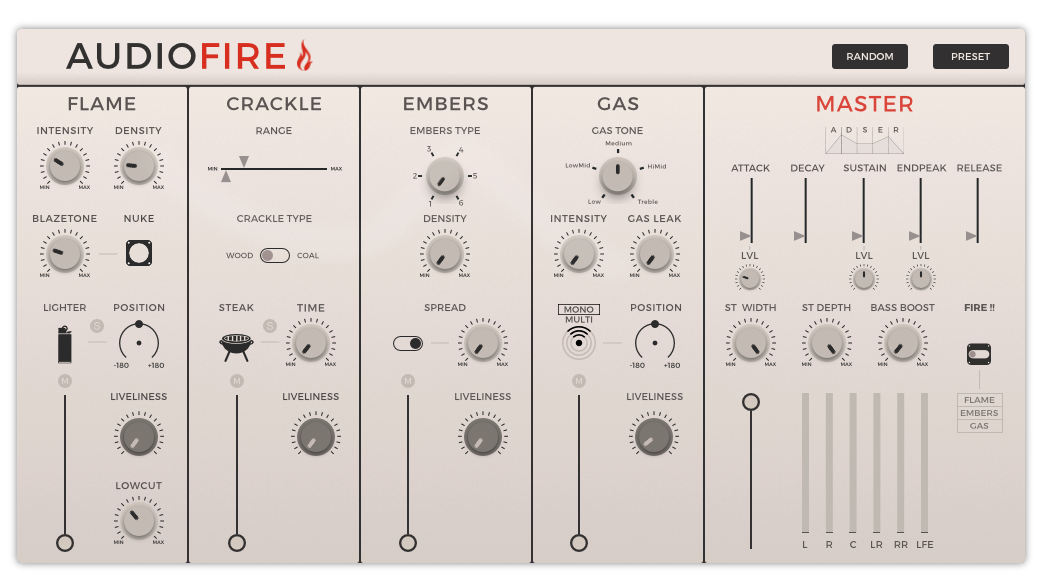
\includegraphics[scale=0.12]{AudioFire_screen.png}
	\caption{Audiofire: audio plug-in that recreates fire sound}
	\end{figure}
  \end{itemize}
\end{frame}

%-------------------------------------------------------
\subsection{Objective}
\begin{frame}{Introduction}{Objective}
%-------------------------------------------------------


  \begin{itemize}
          \item<1-> We are continuing the Audiogaming long project from 2015 (Emilie Abia, Lili Zheng, Quentin Biache)
\begin{block}{}
\begin{center} {\it Objective} : Synthesizing sounds from their spectrum with a $ FFT^{-1} $ \end{center}
	\begin{figure}
	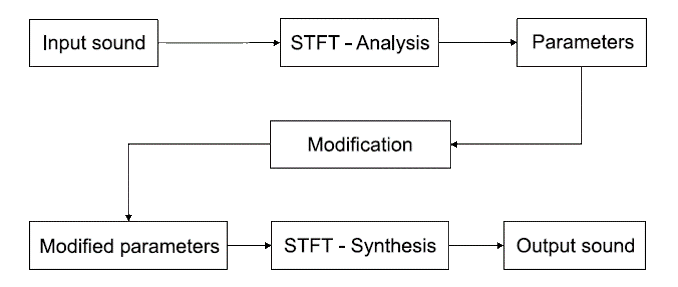
\includegraphics[scale=0.4]{Analysis_Synthesis.png}
	\caption{General approach for modifying a sound in the spectral domain}
	\end{figure}
\end{block}   
	\item<1-> We have to implement a new method of additive synthesis $\Rightarrow$ computationally very fast
  \end{itemize}
\end{frame}

%-------------------------------------------------------
\subsection{Context of the Project}
\begin{frame}{Introduction}{Context of the Project}
%-------------------------------------------------------

  \begin{itemize}
    \item<1-> 6 weeks only $\Rightarrow$ Focus on the synthesis method only.
   \begin{block}{}
	 Given codes in Python and Matlab from the 2015 project :
   \begin{itemize}
 	\item<1-> Python : Analysis estimator of sinus parameters and sinus generation with those parameters (only stationary)
 	\item<1-> Matlab : Some reasearch on the Non-stationary synthesis with the LUT of lobes
   \end{itemize}
   \end{block}   
	\item<1-> We made our own OOP codes in Python
	\item<1-> We have taken the analysis estimator code to test our final synthesis
  \end{itemize}
\end{frame}

%-------------------------------------------------------
\subsection{Work Environment and Project Management}
\begin{frame}{Introduction}{Work Environment}
%-------------------------------------------------------

\begin{figure}
	\centering
	
\includegraphics[scale=0.4]{all_softwares.png}
	\caption{ {\it PyCharm} as Python IDE , {\it Slack} to communicate,{\it GitHub} to stock the codes and have a versionning, {\it Freedcamp} to plan the project events }
\end{figure}
\end{frame}

\begin{frame}{Introduction}{Project Management : Gantt Chart}
%-------------------------------------------------------

\begin{figure}
	\centerline{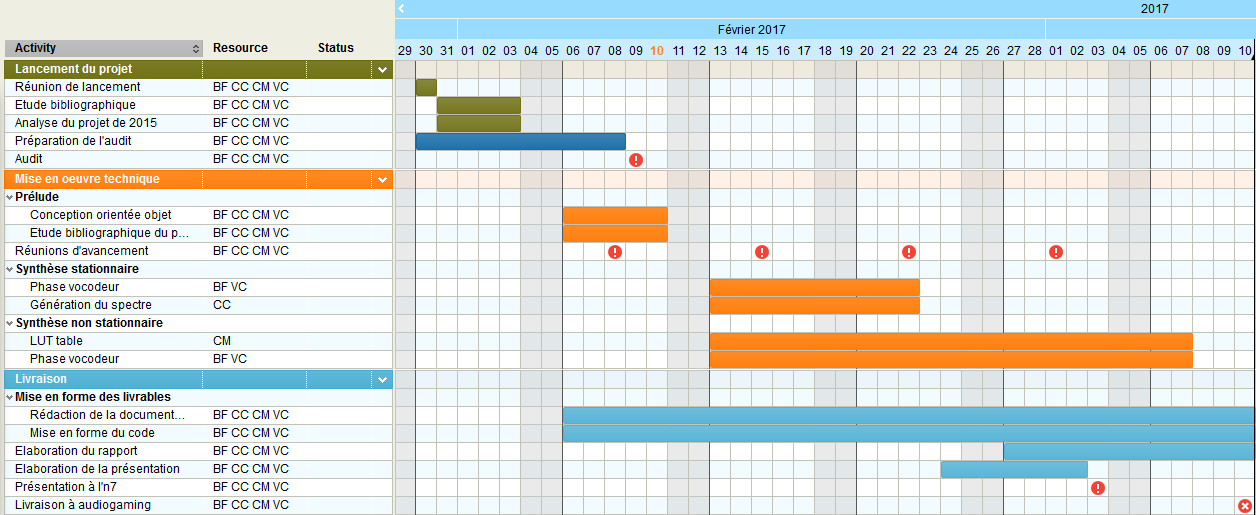
\includegraphics[scale=0.26]{Gantt.png}}
\end{figure}
\end{frame}

%%%%%%%%%%%%%%%%%
%-------------------------------------------------------
\section{Method Overview}
%-------------------------------------------------------
\subsection{Windowing}
\begin{frame}{Method Overview : Analysis}{Windowing}
%-------------------------------------------------------
\begin{figure}
	\centerline
	{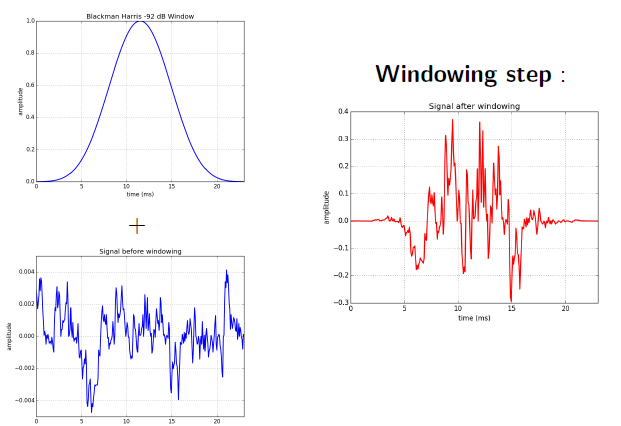
\includegraphics[scale=0.4]{slide1.png}}
	\caption{\it Windowing step}
\end{figure}
\end{frame}
%-------------------------------------------------------
\subsection{Peak Detection}
\begin{frame}{Method Overview : Analysis}{Peak Detection}
%-------------------------------------------------------
Peak detection and extraction of parameters by STPT (particular Short Time Fourier Transform):
\begin{figure}
	\centerline
	{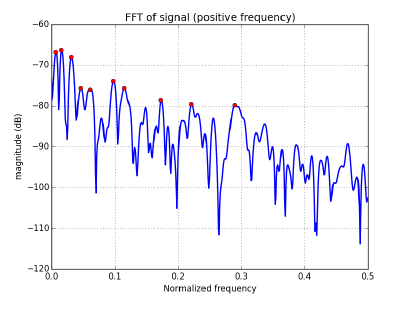
\includegraphics[scale=0.5]{slide2.png}}
	\caption{\it Peak detection}
\end{figure}
\end{frame}
%-------------------------------------------------------
\subsection{Result}
\begin{frame}{Method Overview : Synthesis}{Result}
%-------------------------------------------------------
Additive synthesis according to the parameters from the analysis:
\begin{figure}
	\centerline
	{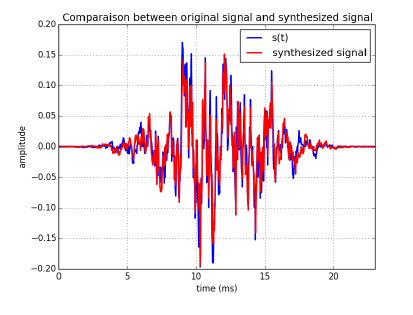
\includegraphics[scale=0.5]{synthesisstep.png}}
	\caption{\it Synthesized signal vs Original signal}
\end{figure}
\end{frame}
%-------------------------------------------------------
\section{The additive synthesis}
%-------------------------------------------------------
\subsection{General approach: The time domain}
\begin{frame}{The additive synthesis}{General approach: The time domain}
%-------------------------------------------------------
\begin{block}{}
The sound signal is represented as a sum of N sinusoids: \\
\centerline{
$ x(t) = \sum\limits_{n=1}^N a_{n} sin(2 \pi f_{n} t + \phi_{n})$}
\begin{itemize}
\item Very costly to implement
\item Impossible to compute in real-time
\end{itemize}
\end{block}
\begin{figure}
	\centerline
	{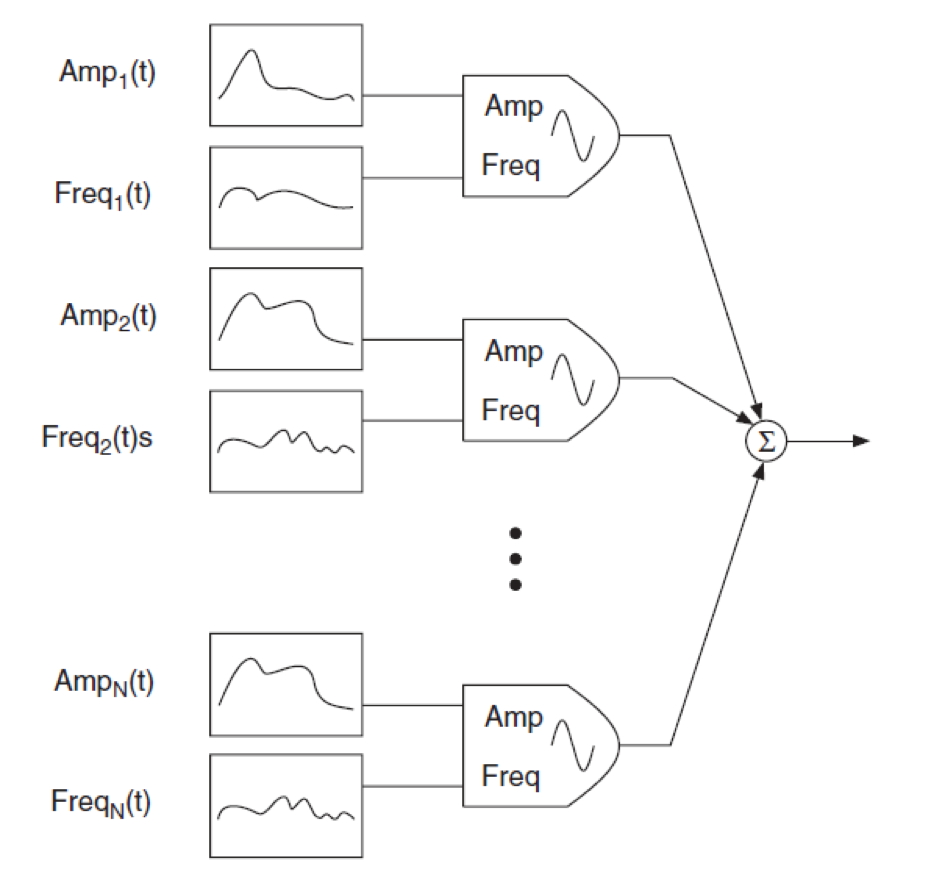
\includegraphics[scale=0.25]{additif.png}}
	\caption{\it The additive synthesis}
\end{figure}
\end{frame}

%-------------------------------------------------------
\subsection{General approach: The frequency domain}
\begin{frame}{The additive synthesis}{General approach: The frequency domain}
%-------------------------------------------------------
\begin{block}{}
We generate the sinusoids in frequency domain in order to reduce the computation time : \\

\begin{itemize}
\item Window the signal to maximize the energy in the main lobe
\item We only keep the main lobe for each sine (9 points)
\item We assume that the parameters (amplitude, frequency, phase) are already given by the analysis
\end{itemize}
\end{block}
\begin{figure}
	\centerline
	{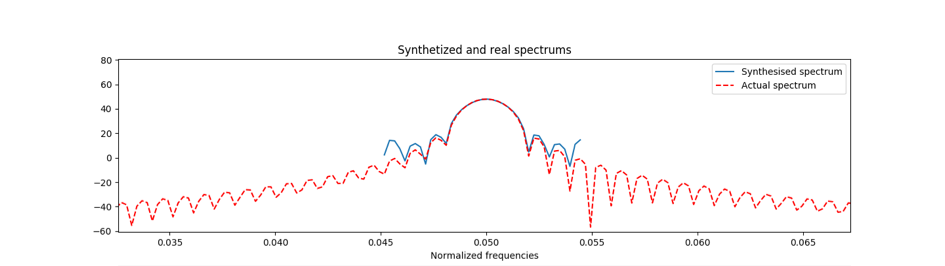
\includegraphics[scale=0.75]{lobe.png}}
	\caption{\it Windowed sine lobe}
\end{figure}
\end{frame}
%-------------------------------------------------------
\subsection{General approach: The frames}
\begin{frame}{The additive synthesis}{The frames}
%-------------------------------------------------------

The sound signal is  a frame-by-frame signal: \\

\begin{figure}

	{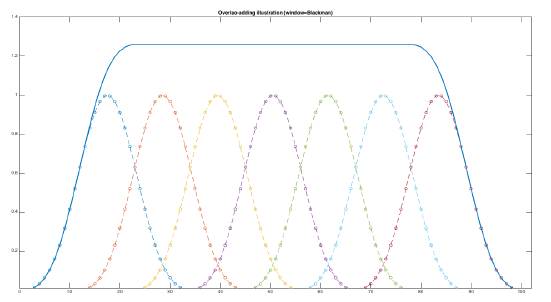
\includegraphics[scale=0.3]{overlap2.png}}
	\caption{\it Sum of small size Hanning windows}
\end{figure}
\begin{figure}
	{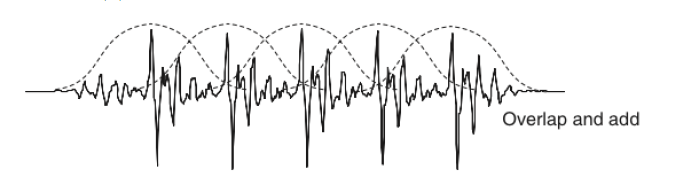
\includegraphics[scale=0.25]{overlap1.png}}
	\caption{\it Overlap and add}
\end{figure}
\end{frame}


%%%%%%%%%%%%%%%%%
\section{Les blocs}

\begin{frame}{Les blocs}

\begin{block}{Bloc simple}
\begin{itemize}
\item Premier point
\item Second point
\item Troisième point
\end{itemize}
\end{block}

\begin{exampleblock}{Bloc exemple}
\begin{itemize}
\item Premier point
\item Second point
\item Troisième point
\end{itemize}
\end{exampleblock}

\begin{alertblock}{Bloc alert}
\begin{itemize}
\item Premier point
\item Second point
\item Troisième point
\end{itemize}
\end{alertblock}
\end{frame}


\section{Les bo\^ites}

\begin{frame}{Les boites}

\begin{columns}

\begin{column}{0.5\textwidth}
\boitejaune{
Ceci est \\
une boite jaune
}

\boiteorange{
Ceci est \\
une boite orange
}

\boitemarron{
Ceci est \\
une boite marron
}
\end{column}

\begin{column}{0.5\textwidth}
\boiteviolette{
Ceci est \\
une boite violette
}

\boitebleue{
Ceci est \\
une boite bleue
}

\boitegrise{
Ceci est \\
une boite grise
}

\end{column}

\end{columns}


\end{frame}



\section{Les listes}
	\subsection{Liste à item}

\begin{frame}{Titre de la frame}

	\begin{itemize}
		\item premier élément de liste,
		\item deuxième élément de liste,
		\item troisième élément de liste.
	\end{itemize}
\end{frame} 

		\subsection{Liste énumérative} 
\begin{frame}{Titre de la frame} 
	\begin{enumerate}
		\item élément de liste numéro 1,
		\item élément de liste numéro 2,
		\item élément de liste numéro 3.  
	\end{enumerate}
\end{frame}


		\subsection{Liste descriptive} 
\begin{frame}{Titre de la frame} 
	\begin{description}
		\item [Thème de présentation : ] ces thèmes sont en fait...
		\item [Thème de couleur : ] gère tout ce qui est couleur...
		\item [Thème de police : ] s'occupe de tout ce qui est police, gras...
		\item [Thème interne : ] s'occupe de l'apparence des éléments...
	\end{description}
\end{frame}



\section{Le texte}

\begin{frame}{Titre de la frame} 

Voici du texte normal

\alert{Voici du texte \texttt{alert}}

\exemple{Voici du texte \texttt{exemple}}

\emph{Voici du texte \texttt{emphase}}

\end{frame}


\section{Les tableaux}

\begin{frame}{Tableaux}

% merci: http://tex.stackexchange.com/questions/112343/beautiful-table-samples

\begin{tcolorbox}[tabjaune,tabularx={X||Y|Y|Y|Y||Y}, boxrule=0.5pt]
Couleur & Prix 1  & Prix 2  & Prix 3   & Prix 4   & Prix 5 \\\hline\hline
Rouge   & 10.00   & 20.00   &  30.00   &  40.00   & 100.00 \\\hline
Vert    & 20.00   & 30.00   &  40.00   &  50.00   & 140.00 \\\hline
Bleu    & 30.00   & 40.00   &  50.00   &  60.00   & 180.00 \\\hline\hline
Orange  & 60.00   & 90.00   & 120.00   & 150.00   & 420.00
\end{tcolorbox}

\begin{tcolorbox}[tabvert,tabularx={X||Y|Y|Y|Y||Y}, boxrule=0.5pt, title=Mon tableau des prix]
Couleur & Prix 1  & Prix 2  & Prix 3   & Prix 4   & Prix 5 \\\hline\hline
Rouge   & 10.00   & 20.00   &  30.00   &  40.00   & 100.00 \\\hline
Vert    & 20.00   & 30.00   &  40.00   &  50.00   & 140.00 \\\hline
Bleu    & 30.00   & 40.00   &  50.00   &  60.00   & 180.00 \\\hline\hline
Orange  & 60.00   & 90.00   & 120.00   & 150.00   & 420.00
\end{tcolorbox}

\end{frame}


\begin{frame}{Tableaux}

% merci: http://tex.stackexchange.com/questions/112343/beautiful-table-samples

\begin{tcolorbox}[tabgris,tabularx={X||Y|Y|Y|Y||Y}, boxrule=0.5pt]
Couleur & Prix 1  & Prix 2  & Prix 3   & Prix 4   & Prix 5 \\\hline\hline
Rouge   & 10.00   & 20.00   &  30.00   &  40.00   & 100.00 \\\hline
Vert    & 20.00   & 30.00   &  40.00   &  50.00   & 140.00 \\\hline
Bleu    & 30.00   & 40.00   &  50.00   &  60.00   & 180.00 \\\hline\hline
Orange  & 60.00   & 90.00   & 120.00   & 150.00   & 420.00
\end{tcolorbox}

\begin{tcolorbox}[taborange,tabularx={X||Y|Y|Y|Y||Y}, boxrule=0.5pt, title=Mon tableau des prix]
Couleur & Prix 1  & Prix 2  & Prix 3   & Prix 4   & Prix 5 \\\hline\hline
Rouge   & 10.00   & 20.00   &  30.00   &  40.00   & 100.00 \\\hline
Vert    & 20.00   & 30.00   &  40.00   &  50.00   & 140.00 \\\hline
Bleu    & 30.00   & 40.00   &  50.00   &  60.00   & 180.00 \\\hline\hline
Orange  & 60.00   & 90.00   & 120.00   & 150.00   & 420.00
\end{tcolorbox}

\end{frame}



\section{Les images}

\begin{frame}{Titre de la frame} 

\begin{figure}
\centering
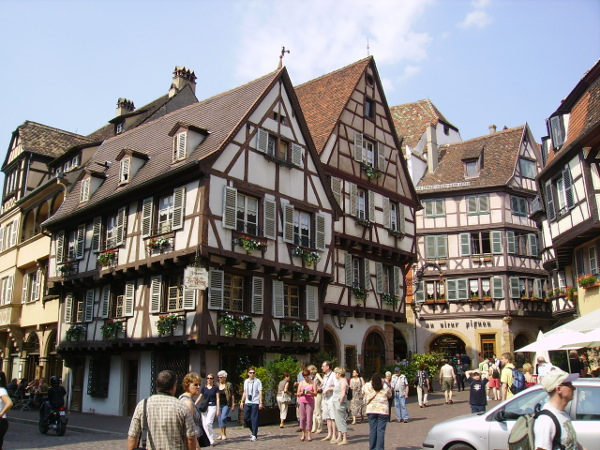
\includegraphics[scale=0.5]{images/architecturebretonne_wikipedia.jpg}
\caption{Éléments d'architecture bretonne typique du Sud de la France. (\href{http://commons.wikimedia.org/wiki/File:Colmar_-_Alsace.jpg}{Wikipédia.fr} CC-By-Sa)}
\end{figure}

\end{frame}



\end{document}
